% Template for ICASSP-2016 paper; to be used with:
%          spconf.sty  - ICASSP/ICIP LaTeX style file, and
%          IEEEbib.bst - IEEE bibliography style file.
% --------------------------------------------------------------------------
\documentclass{article}
\usepackage{spconf,amsmath,graphicx,bm,setspace}
\usepackage{todonotes}
\setlength{\marginparwidth}{1.5cm}
\usepackage{lipsum}
\usepackage{graphicx}
\graphicspath{{images/}}

% ADD THE FOLLOWING COUPLE LINES INTO YOUR PREAMBLE
\let\OLDthebibliography\thebibliography
\renewcommand\thebibliography[1]{
  \OLDthebibliography{#1}
  \setlength{\parskip}{0pt}
  \setlength{\itemsep}{0pt plus 0.3ex}
}

% Example definitions.
% --------------------
\def\x{{\mathbf x}}
\def\L{{\cal L}}

% Title.
% ------
\title{A Knowledge Transfer and Boosting Approach to the Prediction of Affect in Movies}
%
% Single address.
% ---------------
\name{Sabyasachee Baruah$^o$, Rahul Gupta$^+$, Shrikanth Narayanan$^+$}
\address{$^o$Department of Computer Science and Engineering, Indian Institute of Technology, Kharagpur, India \\
$^+$Signal Analysis and Interpretation Lab, University of Southern California, Los Angeles, CA, USA}  
\begin{document}
\ninept
%
\maketitle
%
\begin{abstract}
Affect prediction is a classical problem and has recently garnered special interest in media applications. 
Affect prediction in movies is one such domain, potentially aiding the design as well as the impact analysis of movies.
Given the large diversity in movies (such as different genres and languages), obtaining a comprehensive movie dataset for modeling affect is challenging while models trained on smaller datasets may not generalize. 
In this paper, we address the problem of continuous affect ratings with the availability of limited in domain data resources. 
We initially setup several baseline models trained on in domain data, followed by a proposal of a Knowledge Transfer (KT) + Gradient Boosting (GB) approach.
KT learns models on a larger (although mismatched) data which are then adapted to make predictions on the data of interest. 
GB further updates these predictions based on models learnt from the in domain data.
We observe that the KT + GB models provide Concordance Correlation Coefficient (CCC) values of 0.13 and 0.27 for valence and affect prediction on ACCEDE continuous datasets against best baseline prediction values of 0.12 and 0.11. 
Not only the KT + GB models improve the overall performance metrics, we also observe a more consistent model performance across movies of various genres. 
 
\end{abstract}
%
\begin{keywords}
Gradient Boosting, Knowledge Transfer, affect prediction in movies 
\end{keywords}
%
\section{Introduction}
\label{sec:intro}
Movies are often (if not always) designed to carry a specific emotional impact on its audience \cite{bartsch2012emotional, canini2009emotional}.
Researchers have extended the classical problem of affect prediction to the domain of movies with the goal of understanding the impact of movies as well as aiding the design and analysis of movies \cite{giannakopoulos2009dimensional, jiang2014predicting}. 
Most of the existing algorithms make use of statistical models trained on audio-visual features to predict affective dimensions (e.g. valence and arousal).  
These statistical models often require sufficiently large amounts of data for a low generalization error \cite{vapnik1998statistical}.
Given that movies span a vast variety of genres, are recorded in different languages and even differ from one temporal period to other, comprehensive movie datasets (along with the desired set of annotations) may not always be available to train such statistical models. 
In this paper, we address the problem of continuous affect tracking in movies, with limited availability of in domain data to train low error statistical models. 
We propose a Knowledge Transfer (KT) approach aided with Gradient Boosting (GB) to predict affect in the {\it continuous LIRIS-Annotated Creative Commons Emotional Database for affective video content analysis} ({\it continuous LIRIS-ACCEDE}) database, a dataset with a limited amount of training data.
We train the KT models on a larger (albeit mismatched) dataset, which are later adapted to dataset of interest. 
GB models are trained on a smaller in domain data and operate along with KT models to predict affect induced by movies.
The overarching goal of our experiments is to unify the ongoing efforts in media related research, potentially sharing resources despite inherent incompatibilities. 

Several previous works have investigated the emotional impact of movies \cite{bartsch2010predicting, carroll2010movies}. 
Furthermore, researchers have also applied machine-learning algorithms to both understand and predict emotions induced by movies.
Examples include movie content analysis based on arousal and valence features \cite{xu2008hierarchical}, affect ranking of movie scenes using physiological signals and content analysis \cite{soleymani2008affective} as well as examination of other supervised methods, deep learning and kernel methods within the prediction of affect in movies \cite{malandrakis2011supervised, baveye2015deep}.
Studies have also addressed the issue of robustness in affect prediction using mixture models \cite{goyal2016multimodal} and multimodal learning \cite{pang2015mutlimodal}. 
On the other hand, studies have investigated knowledge transfer (/transfer learning) and have proposed various algorithms as boosting \cite{dai2007boosting}, and transfer learning vis dimensionality reduction \cite{pan2008transfer}.
Knowledge transfer methods have been applied to several domain such as text classification \cite{dai2007transferring} and cross-language classification \cite{ling2008can}.   
In this work, we propose a knowledge transfer approach, aided with gradient boosting, to predict affective dimensions in movies.  
Our approach combines learning from external as well as in domain data resources.
To the best of our knowledge, this is the first such work in movie affect prediction (particularly using data with mismatched in content as well as the annotation protocol and granularity). 

The {\it continuous LIRIS-ACCEDE} dataset consists of 30 movies spanning various genres, languages as well as recording conditions (e.g. color vs black and white vs cartoon).
We initially train various baseline statistical models on the limited in domain dataset to predict the affective dimensions of valence and arousal at a frame rate of 1 value per second.
We analyze the baseline results, observe the performance of models across the movies and motivate the application of KT + GB models.
The KT models are trained on a larger dataset and the model predictions are then adapted to perform prediction on the dataset of interest.
We then propose a GB approach, incorporating KT models as a component.
The GB models are trained sequentially on a pseudo-residual from the previous models and usually are ensemble of weak learners \cite{friedman2001greedy}. 
Our results reflect that KT models, just by themselves, improve upon the conventional in domain statistical models.
Where as the performance for valence saturates using KT models, GB models provide further leverage using in domain data for arousal.
The proposed GB+KT models achieve a Concordance Correlation Coefficient (CCC, a metric accounting for both correlation and bias difference \cite{liao2000note,valstar2016avec}) value of 0.13 and 0.27 on the {\it continuous LIRIS-ACCEDE} dataset for valence and arousal, respectively (against best baseline performances of 0.12 and 0.11).
Further analysis also reveals that not only KT + GB models enhance the performance, but their performances are more consistent across individual movies in the dataset.

We next describe the our dataset of choice in Section 2.
Section 3 describes our methodology and results are presented in Section 4. 
Finally, we present our conclusions and future work in Section 5.

\section{Dataset}

We use the {\it Continuous Annotated Creative Commons Emotional Database for affective video content analysis} ({\it continuous LIRIS-ACCEDE}) dataset for the purpose of our experiments.
This dataset was also used as part of the {\it emotional impact of movies task} organized at the MediaEval challenge 2015 \cite{sjoberg2015mediaeval}.
The dataset consists of 30 short films of length varying from 3 to 28 minutes.
A set of ten annotators rate each movie for the affective dimensions of arousal and valence at a frame rate of 1 sample per second, within a range of -1 to 1.
The final ratings are obtained as frame-wise mean of annotations from each annotator. 
For further information regarding the dataset, we refer the reader to \cite{baveye2015liris}.
In the next section, we describe the features used in our experiments.

\subsection{Feature extraction} \label{feature_extraction}
We use an assembly of visual, speech and music features to train our models.
Table \ref{table:features} shows the list of features along with their frame rate and the extraction toolbox used. 
Note that the frame rates of features from different sources are different.
In order to synchronize the features with the annotations, we extract statistics on the features along a temporal window with a shift of 1 second. 
We extract a set of nine statistics (mean, median, standard deviation, kurtosis, lower and upper quartile, minimum, maximum and range) for every feature. 
Figure~\ref{feat_fig} depicts the extraction of these statistics on the features.
We chose the length of the temporal windows as the one that maximizes the mutual information between the computed features and affect labels (available on the training set).
The mutual information computation assumes a Gaussian distribution for annotations and features, and is borrowed from \cite{mariooryad2015correcting} (Section 4). 
We represent the set of features for a given movie $\mathcal{F}$ as the vector ${\bf X}_{\mathcal{F}} = [X_{\mathcal{F}}(1), .., X_{\mathcal{F}}(n), .., X_{\mathcal{F}}(N) ]$, where $N$ is the total number of analysis frames (equals annotation frames) and $X_{\mathcal{F}}$(n) is the set of audio and video features extracted for analysis frame $n$.
The ground truth annotations are represented as ${\bf t}_{\mathcal F} = [t_\mathcal F(1), .., t_\mathcal F(n), .., t_\mathcal F(N)]$, where $t_\mathcal F(n)$ is the ground truth annotation for the $n^\text{th}$ frame. 

\begin{table}[t]
\centering
\begin{tabular}{@{}l@{}|r|r|r@{}}
{\bf Source} &{\bf Features} & {\bf FPS} & {\bf Toolbox} \\ \hline
Visual & Luminance, intensity & 30 & OpenCV \\ 
       & and optical flow & & \cite{bradski2008learning} \\ \hline
Audio & Mel-frequency cepstral coefficients,& & \\
               & coefficients, voicing probability, & & \\  
               & harmonic to noise ratio, zero crossing & 100 & OpenSmile \\  
               & rate, crossing rate, fundamental & &\cite{eyben2010opensmile} \\  
               & frequency, log energy & & \\ \cline{1-2}
Music & Chroma features (12 semitones) & & \\ 
\end{tabular}
\caption{List of features extracted on the {\it continuous LIRIS-ACCEDE} dataset}
\label{table:features}
\end{table}


\begin{figure}[t]
\centering
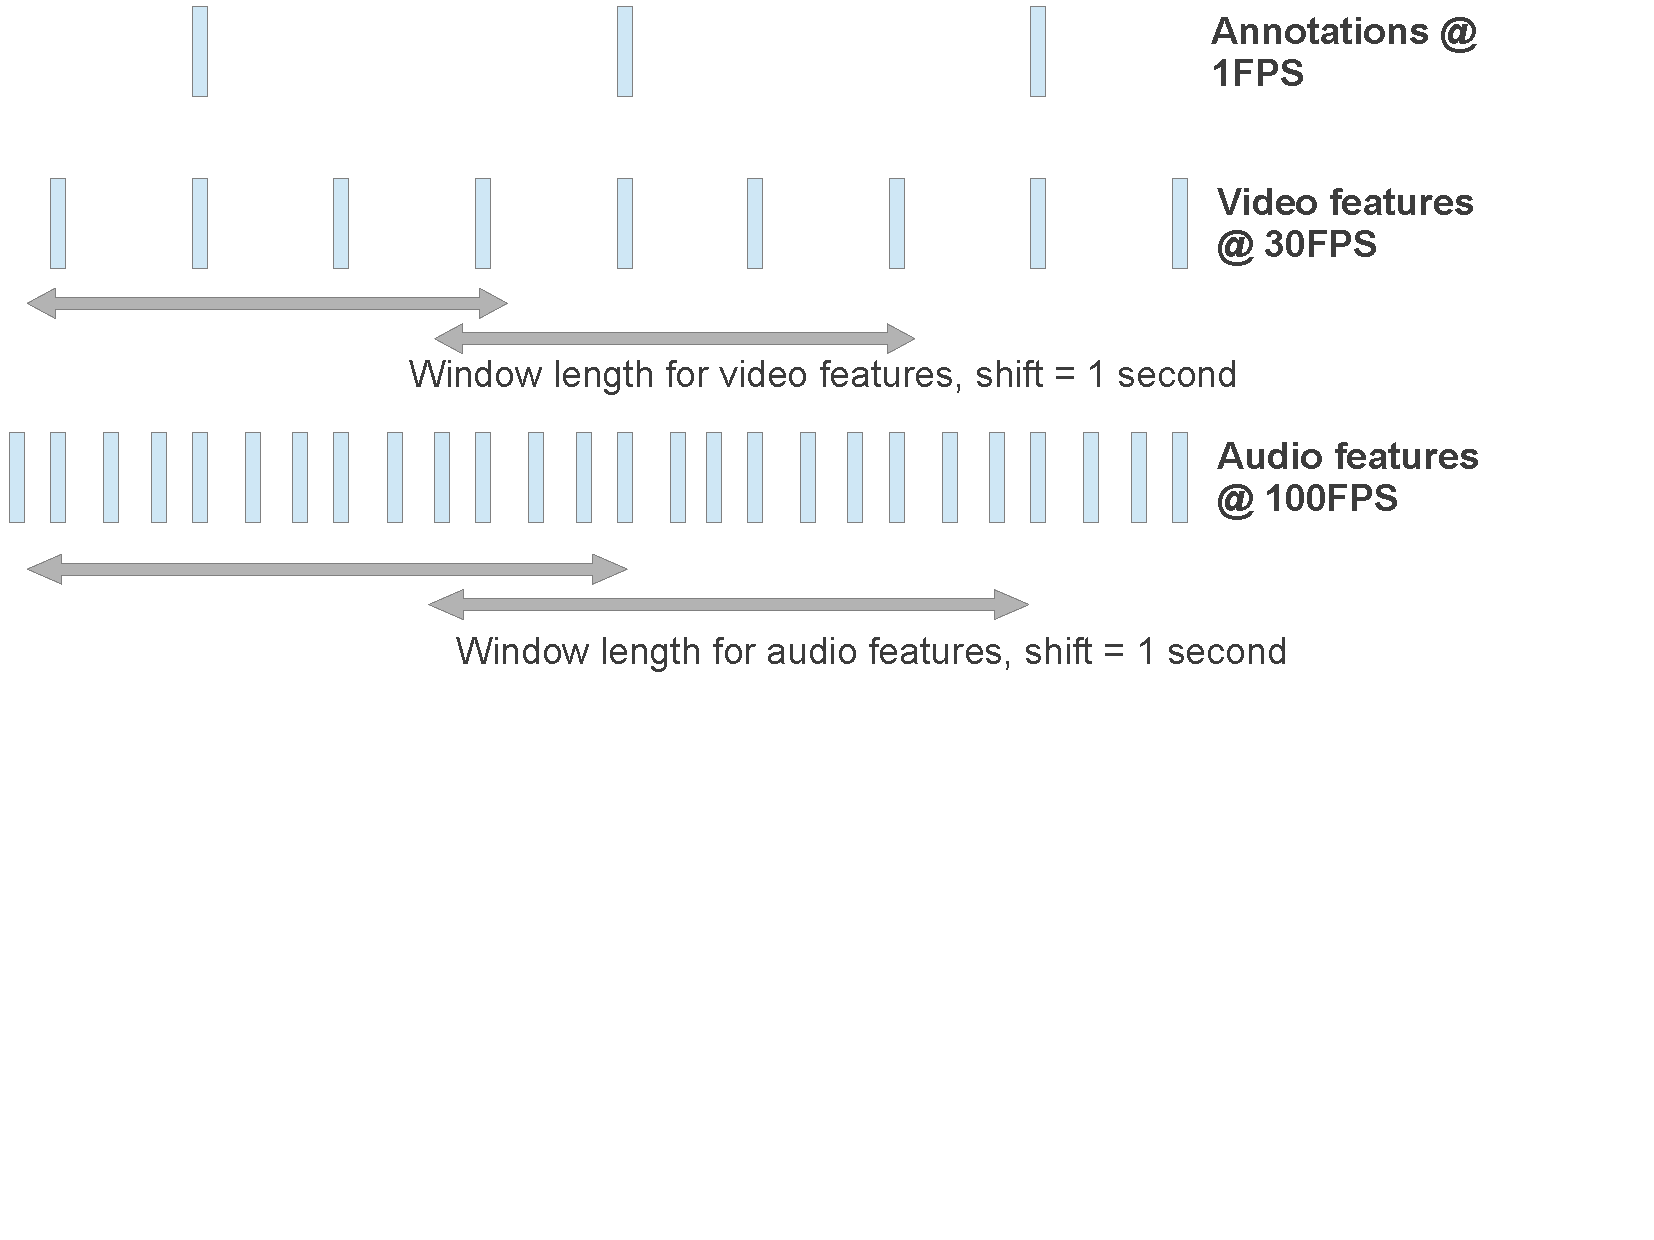
\includegraphics [trim=0cm 9cm 3cm 0cm,clip=true,scale=.35] {images/features_fig.pdf} 
\caption{Feature extraction scheme using extraction of statistics over a temporal window of audio/video frames. Length of temporal window is the one that maximizes mutual information of features with the annotations.}
\label{feat_fig}
\end{figure}


%\indent  A variety of visual, speech and music features are used for training our model. The visual features used are luminance, intensity and optical flow. The speech features are mel-frequency cepstral coefficients, voice probability, zero crossing rate, harmonic to noise ratio, fundamental frequency and energy logarithm. We also include the first and second derivative, and the arithmic mean and standard deviation of the countour of the signal for every speech feature. Lastly we compute 12 semitones for our musical chroma features. We have used the OpenSMILE toolbox for feature extraction. A total of 9 statistics - mean, median, standard deviation, kurtosis, lower and upper quartile, minimum, maximum and range are computed for every feature. We choose a 10 second wide sliding window for calculating our statistics. In total we have 156 visual, speech and musical features, each with nine statistics, thus ending up with a dimension of 1404 for our feature matrix.

\section{Methodology}

We test several regression schemes to predict the continuous valence and affect ratings from the features described in the last section.
Initially, we establish a baseline using multiple regressors.
We discuss the performance of the baseline models and motivate our knowledge transfer and gradient boosting based method.
All our experiments are performed by using a leave one out cross-validation scheme.
During cross-validation, we use 25 movies as the training set, 4 for validation and 1 movie in the test set.
The primary metric for the evaluation of our methods is Concordance Correlation Coefficient (CCC) \cite{liao2000note,valstar2016avec} between the annotated ground truth and the predicted ratings on the test set.
This metric accounts for both the similarity of pattern between the two time series as well as the difference of bias between them. 
Along with this, we also report the correlation coefficient and the Root Mean Square Error (RMSE) between the predicted and the true ratings.
In the next section, we describe the baseline models.

\subsection{Baseline}
%The features and annotations are available at different time frequencies. The video and audio features have been extracted at a rate of 30 and 100 values per second respectively, whereas the ground truth is annotated for each second. To align both these sequences together, we calculate the aforementioned nine statistics over a sliding window on the feature array and assign the computed feature vector of dimension 1404 to the time second at the center of the window. Concordance correlation coefficient is employed as the evaluation metric. We observe the variation in performance for different models on baseline performance as shown in tables \ref{Valence_table} and \ref{Arousal_table}. 

%Farther analysis of the performance of the baseline models shows the variation in performance across the movies, as shown in figure. The movies in our dataset span a wide variety of genres (figure) and enough training data is not available for each type of movie. One of the examples is the film, \textit{To Claire From Sonny}, which is the only romantic movie in the dataset and thus doesn't match any of the movies in the training set in genre, leading to inaccurate predictions of valence and arousal (shown in the figure). To overcome this problem we require a much larger dataset that should have enough variation to be representative of the different genres of the LIRIS-ACCEDE dataset, but should also be compatible so that the knowledge gathered (trained model) can be used to predict the affective labels in the original dataset.

%To this affect we make use of the Discrete LIRIS-ACCEDE dataset. It contains 9800 short video clips of length 8-12 seconds. The clips have been taken from 160 movies. The ground truth consists of a single global valence and arousal label, unlike the previous dataset, in the range 1 to 5, annotated by 1517 annotators from 89 different countries using crowdsourcing. The differences are shown in table \ref{differences}.

%\indent Farther analysis of the performance of the baseline models shows the variation in performance across the movies, as shown in figure \ref{comparison}. The movies in our dataset span a wide variety of genres (figure \ref{genre}) and enough training data is not available for each type of movie. One of the examples is the film, \textit{To Claire From Sonny}, which is the only romantic movie in the dataset and thus doesn't match any of the movies in the training set in genre, leading to inaccurate predictions of valence and arousal (shown in the figure \ref{comparison}). To overcome this problem we require a much larger dataset that should have enough variation to be representative of the different genres of the LIRIS-ACCEDE dataset, but should also be compatible so that the knowledge gathered (trained model) can be used to predict the affective labels in the original dataset.

We use a set of three regressors (linear regression, ridge regression and neural network) to predict the affect ratings from the features. 
Linear regression \cite{bishop2006pattern} is the simplest of the three regressors and linearly maps the features to the affect ratings.
Like linear regression, ridge regression \cite{bishop2006pattern} also performs a linear mapping.
However the weights for ridge regression are regularized \cite{bishop2006pattern}, a scheme helpful in cases involving limited amount of training data.
We test two version of these schemes: with and without feature selection.
During feature selection, we remove features with absolute value of the correlation coefficient below a certain threshold (tuned on the development set).
Correlation coefficient quantifies the linear relationship between the features and the ratings, therefore removal of features with a low correlation coefficient can potentially boost the performance of linear models such as linear and ridge regression. 
Finally, neural networks \cite{bishop2006pattern} perform a non-linear mapping between the features and the affect ratings. 
We train a neural network with one hidden layer.
The number of neurons is tuned on the development set and they have a sigmoidal activation.
We do not perform the correlation coefficient based feature selection with neural networks as it can model non-linear relations between the features and the final labels. 
Table \ref{Baseline_table} shows the results for the performance of these three baseline regression models (the table is shown in results section for ease of comparison with other methods). 


\subsubsection{Discussion} From the results, we observe that the performance for affect prediction varies across the three models.
Particularly, the best performing models are different for the two dimensions.
Neural network regressor performs the best for valence, while linear regression with feature selection performs the best for arousal.
We further list the performances for each movie as obtained using the best regressors for both arousal and valence in Figure~\ref{comparison}. 
The figure shows that the performance per movie varies quite a bit, indicating high error variation depending upon the movie at hand. 
For further analysis, we show the histogram of movie genre distribution in the {\it continuous LIRIS-ACCEDE} dataset in Figure~\ref{genre}.
We observe that certain genres are poorly represented in the dataset, for instance, romance.
This is also reflected in our results as the trained models do not perform well on the only romantic movie ``To Claire from Sonny" (marked in Figure~\ref{comparison}) as the CCC for both arousal and valence prediction is negative for this movie. 
This analysis reflects that a limited data representation despite large diversity in our dataset affects the robustness of the baseline models.
We propose a knowledge transfer + gradient boosting methodology to address this problem, as is discussed in the next section.


\begin{figure*}[t]
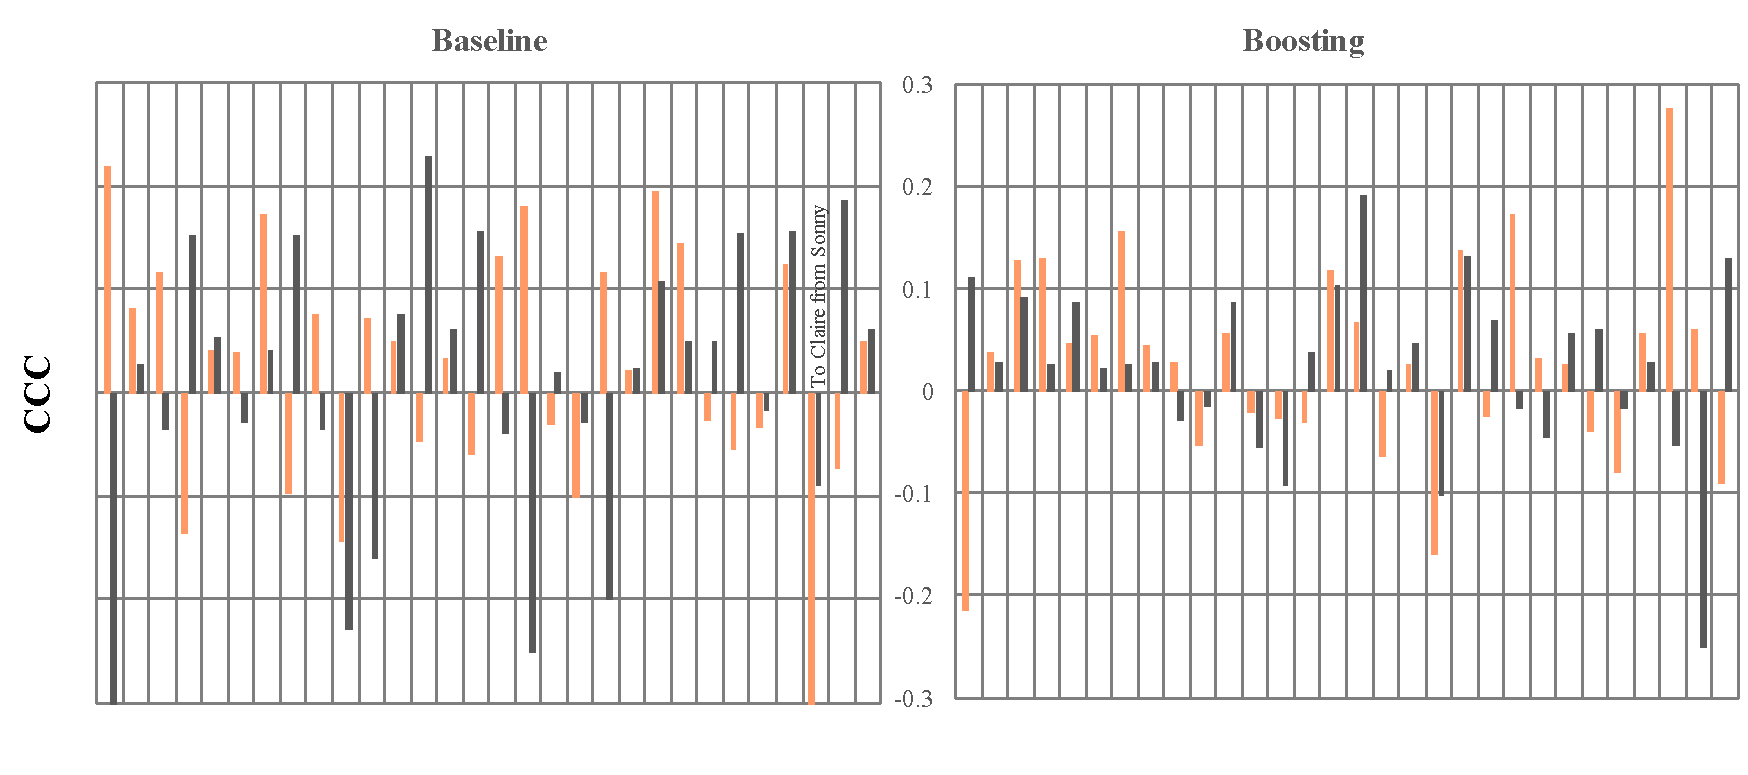
\includegraphics[width=\textwidth, height = 6cm]{images/comparison2.pdf}
\centering
\vspace{-11mm}
\caption{Performance of the best baseline model (left) and KT + GB method (right) across the 30 movies in the {\it continuous LIRIS-ACCEDE} dataset. A more variation in performance is observed for the baseline models.}
\label{comparison}
\end{figure*}

\begin{figure}[t]
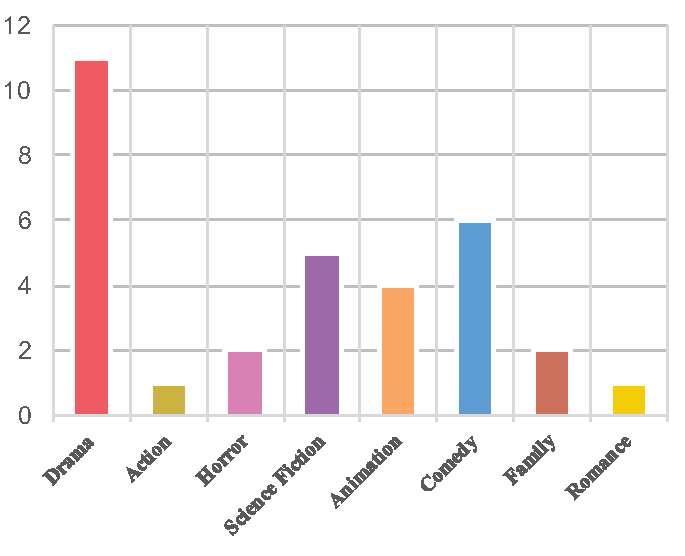
\includegraphics[width=7cm]{genre2}
\centering
\caption{Distribution of genre in {\it continuous LIRIS-ACCEDE} dataset}
\label{genre}
\end{figure}

\begin{table}[t]
\centering
\begin{tabular}{l|p{2.2cm}|p{2.2cm}}
				& Continuous LIRIS-ACCEDE	& Discrete LIRIS-ACCEDE \\ \hline
Duration			& 3 - 28 minutes			& 8 - 12 seconds		\\ \hline	
Annotation granularity & Continuous (1 value/second)				& Global 				\\ \hline
Range			& -1 to 1					& 1 to 5				\\ 
\end{tabular}
\caption{Differences between {\it continuous LIRIS-ACCEDE} and {\it discrete LIRIS-ACCEDE}.}
\label{differences}
\end{table}

\subsection{Proposed method}
As observed from the results and analysis in the previous section, we need to address the problem of limited data leading to poor generalization of our models.
In this section, we propose a knowledge transfer combined with a gradient boosting approach to address the aforementioned issue.
During knowledge transfer, we borrow information learnt on a larger (albeit mismatched) dataset for affect prediction on the dataset of interest.
This is followed by gradient boosting, where we combine models learnt on the {\it continuous LIRIS-ACCEDE} with the existing knowledge transfer models.
We discuss these proposed models in detail below. 

\subsection{Knowledge Transfer (KT)}
During Knowledge Transfer (KT), we train models on a another dataset and operate them on the {\it continuous LIRIS-ACCEDE} dataset to obtain the affect ratings.
To this effect, we use the {\it discrete LIRIS-ACCEDE} dataset consisting of a larger set of ~10k movie clips.  
The {\it discrete LIRIS-ACCEDE} dataset is different from the {\it continuous LIRIS-ACCEDE} dataset in several respects, as shown in Table \ref{differences}.
The discrete dataset consists of small movie clips (~10 seconds in length) as opposed to the continuous dataset (3-28 mins in length).
Furthermore, the annotations are provided at the global scale with a single valence and arousal rating for each clip.
The annotations are in the range of 1-5 as opposed to the scale of -1 to 1 in the continuous dataset. 
We describe the model training on the discrete dataset and application on continuous dataset in detail below.

\subsubsection{KT model training}
Initially, we extract the same of set of features on the discrete dataset as mentioned in the Table~\ref{table:features}.
However, we compute the statistics (listed in section~\ref{feature_extraction}) over the entire duration of the clip (unlike the window-wise approach for {\it continuous LIRIS-ACCEDE} dataset).
We then train a ridge regression model on the feature statistics to predict the discrete ratings.

\subsubsection{KT model application}
In order to apply the model trained on the discrete dataset, we re-use the feature assembly in Table~\ref{table:features}.
However the feature statistics are computed over a fixed window length of 10 seconds with a shift of 1 second (please refer to Figure~\ref{feat_fig}). 
This window length is empirically chosen to match the length of clips in the discrete dataset. 
We then predict the affective dimensions per second using the model trained in the last step.
One can view this operation as making global affect prediction on a sliding window of the continuous data using the KT model.
Since the annotation scales are different for each dataset, we chose to linearly scale the ratings predicted by the knowledge transfer model.
We obtain the predictions using the KT model on the training set and learn a linear scaling such that the minimum mean squared error between the KT model predictions and the true ratings is minimized.
This scaling is then applied on the testing set during evaluation. 
After the KT step, we train a gradient boosting model as discussed in the next section. 

%We extract the same set of features for the short video clips of Discrete LIRIS-ACCEDE as we had done for the movies of Continuous LIRIS-ACCEDE. We train a model on the 9800 videos and predict single values of valence and arousal for each second for the movies. To scale the predictions from the range $[1,5]$ to $[-1,1]$, we use linear modeling by minimizing the squared error between the true labels and predictions. 

\subsection{Gradient boosting (GB)}
%We have used the knowledge gathered from the videos of Discrete LIRIS-ACCEDE to predict the labels of a different dataset, Continuous LIRIS-ACCEDE. However the huge difference in duration between the video clips and movies means that the model cannot still account for the effect of past scenes on the emotions felt by the viewer at the moment. Knowledge transfer predicts the sequence of labels based only on the feature vector of the corresponding second. We leverage the features of the movies to take care of the effect of history while experiencing emotions in viewing a movie.

%We calculate the pseudo-residual error, the difference of the predictions of knowledge transfer and the ground truth. This difference sequence becomes our new target and we train a model on the feature matrix of the movies to predict it. To account for the effect of history on the current annotation of valence and arousal, we shift our feature matrix forward in time relative to the target vector. The delay is found out by maximising mutual information between the shifted feature matrix and target vector. We additionally apply a smooting average filter on our predictions to subtract any noise present in the movie features. We add our predictions of the pseudo-residual error to the output of knowledge transfer to get our new predictions. This process is repeated again until we no longer see an improvement in performance.

The goal of GB model is to extract information from the smaller set of {\it continuous LIRIS-ACCEDE} dataset and incorporate it along with the outputs from the KT model for final affect prediction.
We use the gradient boosting approach similar to the one proposed by Gupta et al. \cite{gupta2015affect} for our experiments.
Gupta et al. \cite{gupta2015affect} proposed an approach using linear filters as base learners to predict continuous affect in music. 
We use a modified approach, where we minimize mean squared error using linear regression on the features statistics after introducing a temporal delay.
We refer the reader to \cite{friedman2001greedy,gupta2015affect} for the details of gradient boosting in minimizing the mean squared error and briefly describe the GB model used in our experiments below. 

\subsubsection{Gradient boosting algorithm for affect prediction}
The proposed gradient boosting learns an ensemble of $k+1$ base learners $\{h_0, h_1, .., h_k\}$, represented as $\bf M_k$. 
For the set of features ${\bf X}_{\mathcal F}$ for the movie $\mathcal F$, the affective predictions $\bf M_k(X_{\mathcal F})$ are computed as  

\begin{equation}
\bm M_k(\bm X_{\mathcal F}) = \sum_{k=0}^K \tilde{\bm h}_k(\bm X_\mathcal F)
\end{equation}

where $\tilde{\bm h}_k(\bm X_\mathcal F)$ is the prediction from the $k^\text{th}$ base learner.
Each of these base learners are learnt using the following algorithm.
\\

\noindent$\bullet$ The base model $\bm M_0 = \tilde{\bm h}_0$ is set as the KT model. Hence the predictions $\bm M_0(\bm X_\mathcal F)$ are as obtained from the KT model mentioned in the previous section. 
The subsequent predictions in the next steps are added $\bm h_0(\bm X_\mathcal F)$ in a boosting fashion, therefore allowing for an integration of knowledge learnt from KT and current data.\\ 

\noindent $\bullet$ For k = 1 to K 

\begin{itemize}
\item[--] Compute the pseudo-residuals ${\bm r}_{\mathcal F}^k = [r^k_\mathcal F(1), .., r^k_\mathcal F(n), .., $ $r^k_\mathcal F(N)]$ for each movie $\mathcal F$ in the training set, where	

\begin{equation} \label{pseudores}
\begin{aligned}
\hspace{-3mm}\bm r^k_\mathcal F &= - { \frac {\partial \Big({\frac{1}{2}\big|\big| \bm t_\mathcal F - {\bm M}_k (\bm X_\mathcal F)\big|\big|^2_2}\Big)} {\partial {\bm M}_k\big({\bm X}_\mathcal F\big)} \bigg|}_{\substack{{\text{at }{\bm M}({\bm X}_\mathcal F) =} \\ {{\bm M}_k({\bm X}_\mathcal F)}}}\\
&= \bm t_\mathcal F - \bm M_k\big( \bm X_\mathcal F \big)
\end{aligned}
\end{equation}

\item[--] Compute a temporal shift in the features that maximizes the mutual information between the shifted features and the pseudo-residuals.
The shift is computed using Gaussian assumption and methodology suggested in \cite{mariooryad2015correcting} (Section 4).

\item[--] Train a linear regressor as the base learner $\bm h_k$ to predict the pseudo-residual using shifted features.

\item[--] Compute weight $\gamma_k$ for the $k^\text{th}$ base leaner using the following one-dimensional optimization problem. $\gamma_k$ is the weight used to scale the outputs from the $k^\text{th}$ base learner.
\begin{equation}
\hspace{-3mm}\gamma_k = \arg\min_{\gamma} \hspace{-4mm} \sum_{\substack{{\mathcal F \in} \\ {\text{training set}}}}\hspace{-2mm} \big|\big| \bm t_\mathcal F - \Big( \bm M_{k-1} (\bm X_\mathcal F) + \gamma \times \bm h_k(\bm X_\mathcal F)\Big) \big|\big|^2_2
\end{equation} 

\item[--] Update the model. 
\begin{equation}
\begin{aligned}
\bm M_k(\bm X_\mathcal F) = \bm M_{k-1} (\bm X_\mathcal F) + \tilde{\bm h}_k(\bm X_\mathcal F) = \\
\bm M_{k-1} (\bm X_\mathcal F) + \big(\gamma_k \times \bm h_k(\bm X_\mathcal F)\big)
\end{aligned}
\end{equation}

\end{itemize}

We summarize the results of the KT and GB models and discuss them in the next section.
The GB models incorporates KT model and is referred to as KT + GB model.

%The performance of the baseline models, knowledge transfer and gradient boosting are shown in tables \ref{Valence_table} and \ref{Arousal_table}. We can observe the improvement in performance of 
%
%\subsection{Discussion}

%\begin{table}[h]
%\centering
%\begin{tabular}{|l|l|l|l|}
%\hline
%						& RMSE		& Correlation 	& CCC 	 \\ \hline
%Linear 					& 0.344		& 0.143		& 0.058  \\ \hline	
%Linear (feature selection)		& 0.339		& 0.200 		& 0.075	 \\ \hline
%Ridge					& 0.344 		& 0.122		& 0.039	 \\ \hline
%Ridge (feature selection)		& 0.344		& 0.121		& 0.044	 \\ \hline
%NN						& 0.330		& .363		& 0.116 \\ \hline
%& & & \\ \hline
%Knowledge transfer 		& 0.331		& 0.295		& \textbf{0.128}	 \\ \hline
%Gradient boosting 			& 0.342 		& 0.208 		& \textbf{0.128}  \\ \hline
%\end{tabular}
%\caption{Results for Valence. The bold numbers shows the improvement.}
%\label{Valence_table}
%\end{table}
%
%\begin{table}[h]
%\centering
%\begin{tabular}{|l|l|l|l|}
%\hline
%						& RMSE		& Correlation 	& CCC 	 \\ \hline
%Linear					& 0.286		& 0.171		& 0.064  \\ \hline	
%Linear (feature selection)		& 0.278		& 0.305 		& 0.113	 \\ \hline
%Ridge					& 0.288  		& 0.141		& 0.030	 \\ \hline
%Ridge (feature selection)		& 0.279		& 0.293		& 0.097	 \\ \hline
%NN						& 0.296		& 0.092		& 0.023 \\ \hline
%& & & \\ \hline
%Knowledge transfer 		& 0.299		& 0.249 		& \textbf{0.221}	 \\ \hline
%Gradient boosting 			& 0.277 		& 0.334 		& \textbf{0.270}  \\ \hline
%\end{tabular}
%\caption{Results for Arousal. The bold numbers shows the improvement.}
%\label{Arousal_table}
%\end{table}

%\begin{table}[t]
%=======
%The performance of the baseline models, knowledge transfer and gradient boosting are shown in tables \ref{Valence_table} and \ref{Arousal_table}. Figure \ref{comparison} compares the performance of baseline models and gradient boosting technique, in both valence and arousal, across the 30 movies of the LIRIS-ACCEDE dataset. \textit{To Claire From Sonny} is a movie from the dataset and has been labelled in the figure. Figure \ref{genre} shows the distribution of genres in the same dataset.

\section{Results and discussion}
Table~\ref{KT_table} shows the results for KT and GB models, along with the baseline results in Table~\ref{Baseline_table}.
From the results, we observe that the KT model by itself outperforms all of the baselines.
This indicates that the affect modeling from a larger (and mismatched) dataset outperforms the models learnt on a smaller dataset (although with matched conditions). 
Further model training using GB incorporating KT model as the first base learner improves performance for arousal. 
However, an improvement is not observed for valence prediction.
This may indicate that valence prediction based on the limited amount of in domain data does not improve the performance beyond that predicted by the KT model.
We perform further analysis regarding the performance of the models on each movie individually, and present our findings. 

\begin{table}[t]
\centering
\caption{Results for affect prediction using the baseline regressors. The best performances for each dimension are shown in bold. FS indicates training with feature selection.}
\begin{tabular}{@{}l|l|l@{}}
\hline
				        & \multicolumn{2}{c}{CCC ($\rho$/ RMSE)}\\ \cline{2-3}
				        & Valence       & Arousal \\ \hline
Linear regression& 0.06 (0.14/ 0.34) & 0.06 (0.17/ 0.29) \\ 
Linear regression + FS & 0.07 (0.20/ 0.34) & {\bf 0.11 (0.30/ 0.28)} \\ 
Ridge regression & 0.04 (0.12/ 0.34) & 0.03 (0.14/ 0.29) \\ 
Ridge regression + FS & 0.04 (0.12/ 0.34) & 0.10 (0.29/ 0.28) \\ 
Neural networks& {\bf 0.12 (0.36/ 0.33)} & 0.02 (0.09/ 0.30) \\ 
\end{tabular}
\label{Baseline_table}
\caption{Results for affect prediction using the KT + GB models.} 
\begin{tabular}{@{}l|l|l@{}}
\hline
				        & \multicolumn{2}{c}{CCC ($\rho$/ RMSE)}\\ \cline{2-3}
				        & Valence       & Arousal \\ \hline
Knowledge transfer\;\;\;\;\;& 0.13 (0.30/ 0.33) & 0.22 (0.25/ 0.30) \\ 
Gradient boosting& 0.13 (0.21/ 0.34) & 0.27 (0.33/ 0.28) \\ 
\end{tabular}
\label{KT_table}
\end{table}

\subsection{Discussion}
%We can observe the improvement in performance of Knowledge Transfer and Gradient Boosting compared to the baseline models. Among the baseline models, we observe that the linear models perform best for arousal, whereas neural networks show the best performance in valence prediction. There is no significant improvement for Gradient Boosting over Knowledge Transfer for valence prediction. When we analyze the performance farther across the movies, we observe a more consistent performance for both valence and arousal for gradient boosting compared to baseline. The case of the movie \textit{To Claire From Sonny} has already been discussed, and we can see the improvent in CCC after gradient boosting.

In order to compare with the per-movie performance of the baseline system, we present the performance of the KT + GB model in Figure~\ref{comparison} for each movie individually.
From the figure, we observe that the performance of the movies is more consistent in the KT + GB models, with fewer movies with a negative CCC in arousal and valence.
Further, we compared the standard deviations of per-movie arousal ($\sigma_\text{aro}$) and valence ($\sigma_\text{val}$) performances between the baseline and KT + GB models ($\sigma$ computed over arousal and valence CCC for the 30 movies). 
The ($\sigma_\text{aro}$) computed over KT + GB model predictions is significantly lower than when computed over the best baseline model (F-test, p-value $<$ 5\%). 
Although, the reduction in ($\sigma_\text{val}$) using GB models over the best baseline model is not significant (F-test, p-value = ??), we do observe a marginal decrease. 

Overall, our experiments suggest that using KT + GB models outperform the baseline models and the motivation for their use lies in the limited availability of in domain data.
Our models not only improve the performance in affect prediction, they are also more consistent in predicting affect across the movies in the dataset, drawn from various genres.
In the next section, we present our conclusions and a few future directions.

\section{Conclusion}
%Knowledge Transfer from a larger and more varied dataset not only improves performance, but also results in more consistent CCC values for different movies. We have used root mean squared error as a proxy for the evaluation of pseudo-residual error for now. We endeavour to use CCC instead in the farther work. 

Research has extended affect prediction to predict the emotional impact of movies, potentially aiding design and analysis of movies.
However, statistical models often require large amounts of data to achieve low error performance. 
This issue is further complicated by the vast diversity in movies.
We propose a KT + GB approach in this paper to address this issue.
KT models borrow knowledge from other larger dataset and GB models incorporate KT models along with models learnt on the in domain data. 
We not only demonstrate the superior performance of KT + GB models on the {\it continuous LIRIS-ACCEDE} dataset, but also achieve a more consistent performance across movies.

In the future, we aim to extend the current work other time series data for media analysis such as interestingness \cite{chen2011violence} and event prediction \cite{butterfield2012interestingness}. 
From the point of view of modeling, we aim to explore other options such as incorporating CCC as a direct optimization cost, exploring other modeling schemes (e.g. neural networks) within the KT + GB models.
Finally, we also aim to extend the models to other domains with similar issues such as affect in music \cite{broekens2010real} and engagement prediction \cite{gupta2016analysis}. 

\footnotesize{
\begin{spacing}{.95 }
%\vfill\pagebreak
% BiBTeX files (here: strings, refs, manuals). The IEEEbib.bst bibliography
% style file from IEEE produces unsorted bibliography list.
% -------------------------------------------------------------------------
\bibliographystyle{IEEEbib2}
\bibliography{refs,strings}
\end{spacing}
}
\end{document}
